\documentclass[11pt]{article}

\usepackage{etex}
\usepackage{tikz}
\usetikzlibrary{calc,arrows,shapes,chains,matrix,positioning,scopes,decorations.pathmorphing,shadows,fit,mindmap}

\usepackage{amssymb}
%%%%%%% Arrows %%%%%%%%%%%%%%%%%%%%%%%%%%%%%%%%%%%%%%%%%%%%%%%%%

\makeatletter
\def \rightarrowfill{\m@th\mathord{\smash-}\mkern-6mu%
  \cleaders\hbox{$\mkern-2mu\mathord{\smash-}\mkern-2mu$}\hfill
  \mkern-6mu\mathord\rightarrow}
\makeatother
\makeatletter
\def \leftarrowfill{\m@th\mathord{\smash-}\mkern-6mu%
  \cleaders\hbox{$\mkern-2mu\mathord{\smash-}\mkern-2mu$}\hfill
%  \mkern-6mu\mathord
}
\makeatother
\makeatletter
\def \Rightarrowfill{\m@th\mathord{\smash=}\mkern-6mu%
  \cleaders\hbox{$\mkern-2mu\mathord{\smash=}\mkern-2mu$}\hfill
  \mkern-6mu\mathord\Rightarrow}
\makeatother

% for labels over and under arrows
%\def \overunderstackrel#1#2#3{\mathrel{\mathop{#1}\limits^{#2}_{#3}}}
%\def\overunderstackrel#1#2#3{\mathrel{\mathop{#1}
%      \limits^{#2}_{\raisebox{.6ex}{\hbox {$#3$}}\raisebox{-.4ex}{\hbox{}}}}}
\def \overunderstackrel#1#2#3{\mathrel{\mathop{#1}\limits^{#2}_{\raisebox{.8ex}
{$\scriptstyle #3$}\raisebox{-.2ex}{\hbox{}}}}}
\def \overstackrel#1#2{\mathrel{\mathop{#1}\limits^{#2}}}
\def \understackrel#1#2{\mathrel{\mathop{#1}\limits_{#2}}}

\def\ured{\rightarrow}
\def\tred#1{\overstackrel{\rightarrowfill}{#1}}
\def\iured#1{\rightarrow_{\descr{\scriptsize #1}}}
\def\itred#1#2{\mathrel{{\overstackrel{\rightarrowfill}{#2}}_{\descr
  {\scriptsize #1}}}}
\def\tr#1{\overstackrel{\rightarrowfill}{#1}}
\def\act#1#2{#1 @ #2}
\def\actr#1#2{\overstackrel{\rightarrowfill}{\act {#1}{#2}}}
\def\iactr#1#2#3{\overstackrel{\rightarrowfill}{\act {#2}{#3}}_{\descr
  {\scriptsize #1}}}

%%%%%%% New Environments %%%%%%%%%%%%%%%%%%%%%
\def\introrule{{\cal I}}\def\elimrule{{\cal E}}%%
\def\andintro{\using{\land}\introrule\justifies}%%
\def\impelim{\using{\Rightarrow}\elimrule\justifies}%%
\def\allintro{\using{\forall}\introrule\justifies}%%
\def\allelim{\using{\forall}\elimrule\justifies}%%
\def\falseelim{\using{\bot}\elimrule\justifies}%%
\def\existsintro{\using{\exists}\introrule\justifies}%%

%% #1 is meant to be 1 or 2 for the first or second formula
\def\andelim#1{\using{\land}#1\elimrule\justifies}%%
\def\orintro#1{\using{\lor}#1\introrule\justifies}%%

%% #1 is meant to be a label corresponding to the discharged hypothesis/es
\def\impintro#1{\using{\Rightarrow}\introrule_{#1}\justifies}%%
\def\orelim#1{\using{\lor}\elimrule_{#1}\justifies}%%
\def\existselim#1{\using{\exists}\elimrule_{#1}\justifies}

%%==========================================================================

\newdimen\proofrulebreadth \proofrulebreadth=.04em
\newdimen\proofdotseparation \proofdotseparation=1.25ex
\newdimen\proofrulebaseline \proofrulebaseline=2ex
\newcount\proofdotnumber \proofdotnumber=3
\let\then\relax
\def\hfi{\hskip0pt plus.0001fil}

\mathchardef\squigto="3A3B
%
% flag where we are
\newif\ifinsideprooftree\insideprooftreefalse
\newif\ifonleftofproofrule\onleftofproofrulefalse
\newif\ifproofdots\proofdotsfalse
\newif\ifdoubleproof\doubleprooffalse
\let\wereinproofbit\relax
%
% dimensions and boxes of bits
\newdimen\shortenproofleft
\newdimen\shortenproofright
\newdimen\proofbelowshift
\newbox\proofabove
\newbox\proofbelow
\newbox\proofrulename
%
% miscellaneous commands for setting values
\def\shiftproofbelow{\let\next\relax\afterassignment\setshiftproofbelow\dimen0 }
\def\shiftproofbelowneg{\def\next{\multiply\dimen0 by-1 }%
\afterassignment\setshiftproofbelow\dimen0 }
\def\setshiftproofbelow{\next\proofbelowshift=\dimen0 }
\def\setproofrulebreadth{\proofrulebreadth}

%=============================================================================
\def\prooftree{% NESTED ZERO (\ifonleftofproofrule)
%
% first find out whether we're at the left-hand end of a proof rule

\ifnum  \lastpenalty=1 \then   \unpenalty \else
\onleftofproofrulefalse \fi
%
% some space on left (except if we're on left, and no infinity for outermost)
\ifonleftofproofrule \else   \ifinsideprooftree
        \then   \hskip.5em plus1fil
        \fi
\fi
%
% begin our proof tree environment
\bgroup% NESTED ONE (\proofbelow, \proofrulename, \proofabove,
%               \shortenproofleft, \shortenproofright, \proofrulebreadth)
\setbox\proofbelow=\hbox{}\setbox\proofrulename=\hbox{}%
\let\justifies\proofover\let\leadsto\proofoverdots\let\Justifies\proofoverdbl
\let\using\proofusing\let\[\prooftree
\ifinsideprooftree\let\]\endprooftree\fi
\proofdotsfalse\doubleprooffalse
\let\thickness\setproofrulebreadth
\let\shiftright\shiftproofbelow \let\shift\shiftproofbelow
\let\shiftleft\shiftproofbelowneg
\let\ifwasinsideprooftree\ifinsideprooftree
\insideprooftreetrue
%
% now begin to set the top of the rule (definitions local to it)
\setbox\proofabove=\hbox\bgroup$\displaystyle % NESTED TWO
\let\wereinproofbit\prooftree
%
% these local variables will be copied out:
\shortenproofleft=0pt \shortenproofright=0pt \proofbelowshift=0pt
%
% flags to enable inner proof tree to detect if on left:
\onleftofproofruletrue\penalty1 }

%=============================================================================
% end whatever box and copy crucial values out of it
\def\eproofbit{% NESTED TWO
%
% various hacks applicable to hypothesis list
\ifx    \wereinproofbit\prooftree \then   \ifcase \lastpenalty
        \then   \shortenproofright=0pt  % 0: some other object, no indentation
        \or     \unpenalty\hfil         % 1: empty hypotheses, just glue
        \or     \unpenalty\unskip       % 2: just had a tree, remove glue
        \else   \shortenproofright=0pt  % eh?
        \fi
\fi
%
% pass out crucial values from scope
\global\dimen0=\shortenproofleft \global\dimen1=\shortenproofright
\global\dimen2=\proofrulebreadth \global\dimen3=\proofbelowshift
\global\dimen4=\proofdotseparation
%\global\mscount=\proofdotnumber
%
% end the box
$\egroup  % NESTED ONE
%
% restore the values
\shortenproofleft=\dimen0 \shortenproofright=\dimen1
\proofrulebreadth=\dimen2 \proofbelowshift=\dimen3
\proofdotseparation=\dimen4
%\proofdotnumber=\mscount
}

%=============================================================================
\def\proofover{% NESTED TWO
\eproofbit % NESTED ONE
\setbox\proofbelow=\hbox\bgroup % NESTED TWO
\let\wereinproofbit\proofover
$\displaystyle
}%
%
%=============================================================================
\def\proofoverdbl{% NESTED TWO
\eproofbit % NESTED ONE
\doubleprooftrue
\setbox\proofbelow=\hbox\bgroup % NESTED TWO
\let\wereinproofbit\proofoverdbl
$\displaystyle
}%
%
%=============================================================================
\def\proofoverdots{% NESTED TWO
\eproofbit % NESTED ONE
\proofdotstrue
\setbox\proofbelow=\hbox\bgroup % NESTED TWO
\let\wereinproofbit\proofoverdots


$\displaystyle
}%
%
%=============================================================================
\def\proofusing{% NESTED TWO
\eproofbit % NESTED ONE
\setbox\proofrulename=\hbox\bgroup % NESTED TWO
\let\wereinproofbit\proofusing
\kern0.3em$ }

%=============================================================================
\def\endprooftree{% NESTED TWO
\eproofbit % NESTED ONE
% \dimen0 =     length of proof rule
% \dimen1 =     indentation of conclusion wrt rule
% \dimen2 =     new \shortenproofleft, ie indentation of conclusion
% \dimen3 =     new \shortenproofright, ie
%                space on right of conclusion to end of tree
% \dimen4 =     space on right of conclusion below rule
  \dimen5 =0pt% spread of hypotheses
% \dimen6, \dimen7 = height & depth of rule
%
% length of rule needed by proof above
\dimen0=\wd\proofabove \advance\dimen0-\shortenproofleft
\advance\dimen0-\shortenproofright
%
% amount of spare space below
\dimen1=.5\dimen0 \advance\dimen1-.5\wd\proofbelow \dimen4=\dimen1
\advance\dimen1\proofbelowshift \advance\dimen4-\proofbelowshift
%
% conclusion sticks out to left of immediate hypotheses
\ifdim  \dimen1<0pt \then   \advance\shortenproofleft\dimen1
        \advance\dimen0-\dimen1
        \dimen1=0pt
%       now it sticks out to left of tree!
        \ifdim  \shortenproofleft<0pt
        \then   \setbox\proofabove=\hbox{%
                        \kern-\shortenproofleft\unhbox\proofabove}%
                \shortenproofleft=0pt
        \fi
\fi
%
% and to the right
\ifdim  \dimen4<0pt \then   \advance\shortenproofright\dimen4
        \advance\dimen0-\dimen4
        \dimen4=0pt
\fi
%
% make sure enough space for label
\ifdim  \shortenproofright<\wd\proofrulename \then
\shortenproofright=\wd\proofrulename \fi
%
% calculate new indentations
\dimen2=\shortenproofleft \advance\dimen2 by\dimen1
\dimen3=\shortenproofright\advance\dimen3 by\dimen4
%
% make the rule or dots, with name attached
\ifproofdots \then
        \dimen6=\shortenproofleft \advance\dimen6 .5\dimen0
        \setbox1=\vbox to\proofdotseparation{\vss\hbox{$\cdot$}\vss}
        \setbox0=\hbox{%
                \kern\dimen6
                $\vcenter to\proofdotnumber\proofdotseparation
                        {\leaders\box1\vfill}$%
                \unhbox\proofrulename}%
\else   \dimen6=\fontdimen22\the\textfont2 % height of maths axis
        \dimen7=\dimen6
        \advance\dimen6by.5\proofrulebreadth
        \advance\dimen7by-.5\proofrulebreadth
        \setbox0=\hbox{%
                \kern\shortenproofleft
                \ifdoubleproof
                \then   \hbox to\dimen0{%
                        $\mathsurround0pt\mathord=\mkern-6mu%
                        \cleaders\hbox{$\mkern-2mu=\mkern-2mu$}\hfill
                        \mkern-6mu\mathord=$}%
                \else   \vrule height\dimen6 depth-\dimen7 width\dimen0
                \fi
                \unhbox\proofrulename}%
        \ht0=\dimen6 \dp0=-\dimen7
\fi
%
% set up to centre outermost tree only
\let\doll\relax
\ifwasinsideprooftree \then   \let\VBOX\vbox \else
\ifmmode\else$\let\doll=$\fi
        \let\VBOX\vcenter
\fi
% this \vbox or \vcenter is the actual output:
\VBOX   {\baselineskip\proofrulebaseline \lineskip.2ex
        \expandafter\lineskiplimit\ifproofdots0ex\else-0.6ex\fi
        \hbox   spread\dimen5   {\hfi\unhbox\proofabove\hfi}%
        \hbox{\box0}%
        \hbox   {\kern\dimen2 \box\proofbelow}}\doll%
%
% pass new indentations out of scope
\global\dimen2=\dimen2 \global\dimen3=\dimen3
\egroup % NESTED ZERO
\ifonleftofproofrule \then   \shortenproofleft=\dimen2 \fi
\shortenproofright=\dimen3
%
% some space on right and flag we've just made a tree
\onleftofproofrulefalse \ifinsideprooftree \then   \hskip.5em plus
1fil \penalty2 \fi }

%==========================================================================
% IDEASWe also show an example of interest.
% 1.    Specification of \shiftright and how to spread trees.
% 2.    Spacing command \m which causes 1em+1fil spacing, over-riding
%       exisiting space on sides of trees and not affecting the
%       detection of being on the left or right.
% 3.    Hack using \@currenvir to detect LaTeX environment; have to
%       use \aftergroup to pass \shortenproofleft/right out.
% 4.    (Pie in the sky) detect how much trees can be "tucked in"
% 5.    Discharged hypotheses (diagonal lines).


\newcommand{\labeltree}[3]
{\begin{tabular}{l}
 {#1} \\
 {\prooftree {#2}
 \justifies {#3}
 \endprooftree}
 \end{tabular}
} 
\newcommand{\modif}[1]{\begin{color}{red}#1\end{color}} % To highlight changes
\newcommand{\modiff}[1]{\begin{color}{blue}#1\end{color}} % To highlight changes
\newcommand{\remove}[1]{\begin{color}{green}#1\end{color}} % To highlight changes
%\newcommand{\remove}[1]{} % To highlight changes

\newcommand{\rulelabel}[1]{\textit{\small{(#1)}}} % label for operational semantics rules

%%% Environments and theorems %%%
%\newtheorem{theorem}{Theorem}[section]
%\newtheorem{lemma}{Lemma}[section]
%\newtheorem{corollary}{Corollary}[section]
%\newtheorem{property}{Property}[section]
%\newtheorem{definition}{Definition}[section]
%\newtheorem{remark}{Remark}[section]

%%% Colors %%%
\definecolor{mygray}{rgb}{.90,.90,.90}
\definecolor{myDarkGray}{rgb}{.75,.75,.75}
\definecolor{myLightGray}{rgb}{.965,.965,.965}

\newcommand{\graybg}[1]{\colorbox{mygray}{#1}} % To highlight some parts of a specification

%%% Languges names

\newcommand{\SCEL}{\textsc{SCEL}}
\newcommand{\SCELt}{\textsc{SCEL2}}
\newcommand{\Klaim}{\textsc{Klaim}}
\newcommand{\MetaKlaim}{\textsc{MetaKlaim}}
\newcommand{\kos}{$\mathcal{K}$oS}
\newcommand{\kaos}{\textsc{Kaos}}
\newcommand{\cows}{\textsc{COWS}}
\newcommand{\ccpi}{\textsc{cc-pi}}
\newcommand{\pic}{$\pi$-calculus}

\newcommand{\xmltag}[1]{\mathtt{<\!#1\!>}}
\newcommand{\und}{\_}                       % underscore
\newcommand{\dontcare}{\mathtt{\und}}
\newcommand{\arr}[1]{\langle #1 \rangle}    % for tuples of objects
\newcommand{\arrcomp}{:}
\newcommand{\set}[1]{\{#1\}}
\newcommand{\undef}{\mathbf{undef}} % denota undefined
\newcommand{\false}{\mathbf{false}}
\newcommand{\true}{\mathbf{true}}
\newcommand{\assoc}[2]{#1 \mapsto #2} % associazione variabile-valore
\newcommand{\substi}[1]{\{#1\}}

\newcommand{\delimite}[1]{\mbox{$\overstackrel{\belowfill}{\mbox{$\overstackrel{#1}{\abovefill}$}}$}}
\makeatletter
\def \abovefill{
  {\vrule width0.3mm height 1.8mm depth-0.3mm}
  \leaders\hrule height1.8mm depth-1.5mm\hfill
  {\vrule width0.3mm height 1.8mm depth-0.3mm}}
\makeatother
\makeatletter
\def \belowfill{
  {\vrule width0.3mm height1.5mm}
  \leaders\hrule height0.3mm\hfill
  {\vrule width0.3mm height1.5mm}}
\makeatother

%%% SYNTAX

\newcommand{\actell}{\textbf{tell}}                           %output operation
\newcommand{\acretract}{\textbf{retract}}
\newcommand{\actellp}[4]{\ensuremath{\mathbf{tell}(#1,#2,#3)@#4}}
\newcommand{\acretractp}[4]{\ensuremath{\mathbf{retract}(#1,#2,#3)@#4}}
\newcommand{\acput}{\textbf{put}}                           %output operation
\newcommand{\acout}{\textbf{out}}                           %output operation
\newcommand{\acputp}[2]{\ensuremath{\mathbf{put}(#1)@#2}}   %output operation with parameters
\newcommand{\acputpq}[3]{\ensuremath{\mathbf{put}(#1)@_{#3}#2}}   %output operation with parameters and quality level
\newcommand{\acget}{\textbf{get}}
\newcommand{\acin}{\textbf{in}}
\newcommand{\acgetp}[2]{\ensuremath{\mathbf{get}(#1)@#2}}
\newcommand{\acreadold}{\textbf{read}}
%\newcommand{\acreadp}[2]{\ensuremath{\mathbf{read}(#1)@#2}}
%\newcommand{\acread}{\textbf{rtv}}
\newcommand{\acread}{\textbf{qry}}
%\newcommand{\acreadp}[2]{\ensuremath{\mathbf{rtv}(#1)@#2}}
\newcommand{\acreadp}[2]{\ensuremath{\mathbf{qry}(#1)@#2}}
%\newcommand{\acmove}{\textbf{exec}}
\newcommand{\acexec}{\textbf{exec}}
\newcommand{\aceval}{\textbf{eval}}
%\newcommand{\acmovep}[2]{\ensuremath{\mathbf{exec}(#1)@#2}}
%\newcommand{\acexecp}[2]{\ensuremath{\mathbf{exec}(#1)@#2}}
\newcommand{\acexecp}[1]{\ensuremath{\mathbf{exec}(#1)}}
\newcommand{\acnewold}{\textbf{newloc}}
\newcommand{\acnew}{\textbf{new}}
\newcommand{\acnewp}[1]{\ensuremath{\mathbf{new}(#1)}}
\newcommand{\acfresh}{\textbf{fresh}}
\newcommand{\acfreshp}[1]{\ensuremath{\mathbf{fresh}(#1)}}
\newcommand{\acenforce}{\textbf{enforce}}
\newcommand{\acenforcep}[1]{\ensuremath{\mathbf{enforce}(#1)}}

\newcommand{\procnil}{\ensuremath{\textbf{nil}}}
%\newcommand{\mmif}{\textbf{if}}
%\newcommand{\mmthen}{\textbf{then}}
%\newcommand{\mmelse}{\textbf{else}}
%\newcommand{\mmfor}{\textbf{for}}
%\newcommand{\mmforall}{\textbf{forall}}
%\newcommand{\mmwhile}{\textbf{while}}
%\newcommand{\mmdo}{\textbf{do}}

\newcommand{\naddr}{n}              % network addresses
\newcommand{\naddrbis}{m}              % network addresses
\newcommand{\vaddr}{x}              % variable for network addresses
\newcommand{\nvaddr}{c}          % network addresses or variable
\newcommand{\self}{\mathsf{self}}   % local address
\newcommand{\super}{\mathsf{super}}
\newcommand{\predic}[1]{\mathsf{#1}}

\newcommand{\pair}[1]{\langle #1 \rangle}

\newcommand{\bexpr}{e}               % expressions for basic values

%\newcommand{\conf}[1]{\langle {#1} \rangle}
%\newcommand{\netconf}[2]{ #1 \vdash #2 }
\newcommand{\tuplewp}[2]{#2 \triangleright \langle #1 \rangle}
\newcommand{\tuple}[1]{\langle #1 \rangle}
%\newcommand{\pol}[2]{#2 \triangleright #1}
\newcommand{\pol}{\Pi}          % policies
\newcommand{\rules}{\rho}          % rules

%\newcommand{\parcomp}{\mbox{$ \mid $}}          % parallel among components
\newcommand{\parp}[1]{\parallel_{{}_{#1}}}          % parameterised parallel
\newcommand{\parcompp}{\parp{\pol}}                 % generic policy parameterised parallel
\newcommand{\parcomp}{\parallel}                    % parallel
\newcommand{\choice}{\: + \:}

\newcommand{\ecs}{ {\bf 0 } }                   % empty set of components
\newcommand{\knw}{\mathcal{K}}                      % knowledge representation + management
%\newcommand{\loccomp}[3]{ #1 ::_{{}_{#2}}^{{}_{#3}} }       % component
\newcommand{\loccomp}[2]{ \interf{#1}[#2] }                  % component
\newcommand{\ens}[3]{ #1 ::_{{}_{#2}}^{{}_{#3}} }  % ensemble
%\newcommand{\ens}[2]{ #1[#2] }                      % ensemble
\newcommand{\interf}[1]{\ensuremath{\mathbf{\cal #1}}}
\newcommand{\interfm}[1]{\cal #1}

\newcommand{\enspred}[1]{\mathsf{#1}}

\newcommand{\res}[1]{(\nu #1)}                  % name anonymiser
\newcommand{\reslab}[1]{\nu #1}                  % name anonymiser
\newcommand{\ren}[1]{\{#1\}}                    % name renaming
\newcommand{\penf}[1]{[#1]}                     % policy enforcement
\newcommand{\broadc}[1]{(#1 \rightrightarrows)} % broadcast
\newcommand{\auth}[2]{#1[\,#2\,]}                     % autonomic handling

\newcommand{\defi}{\stackrel{def}{=}}
\newcommand{\define}{\triangleq}
\newcommand{\wt}{\widetilde}

%\newcommand{\sep}{\ \big |\ }
\newcommand{\sep}{\ \ \left|
                      \begin{array}{l}
                      \\
                      \end{array}
                   \right.}

\newcommand{\Act}{{\cal L}}     % set of visible actions

%%% OPERATIONAL SEMANTICS

\newcommand{\valt}[2]{\mbox{${\mathcal E}[\![ \: #1 \: ]\!]_{#2}$}}
%\newcommand{\sub}[2]{\{\raisebox{.5ex}{\small$#1$}\! / \!\mbox{\small$#2$}\}} % name substitution
\newcommand{\sub}[3]{ #1 \{\raisebox{.1ex}{\small$#2$}\! / \!\mbox{\small $#3$}\}} % name substitution
\newcommand{\mumatch}{match}

\newcommand{\n}[1]{{\mathit{n}}(#1)}    % names
\newcommand{\fn}[1]{{\mathit{fn}}(#1)}    % free names
\newcommand{\bn}[1]{{\mathit{bn}}(#1)}    % bound names
\newcommand{\var}[1]{{\mathit{v}}(#1)}    % variables
\newcommand{\fv}[1]{{\mathit{fv}}(#1)}    % free variables
\newcommand{\bv}[1]{{\mathit{bv}}(#1)}    % bound variables

\newcommand{\alfaconv}{=_{\alpha}}
\newcommand{\reduce}{\longmapsto}

\newcommand{\thenstr}{\prlaw{Then}}
\newcommand{\elsestr}{\prlaw{Else}}
\newcommand{\alphastr}{\prlaw{Alpha}}
\newcommand{\callstr}{\prlaw{Rec}}
\newcommand{\defstr}{\prlaw{PDef}}
\newcommand{\ridstr}{\prlaw{RNil}}
\newcommand{\rnodestr}{\prlaw{RNode}}
\newcommand{\rnodepstr}{\prlaw{RNode'}}
\newcommand{\rcomstr}{\prlaw{RCom}}
\newcommand{\pidstr}{\prlaw{PZero}}
\newcommand{\pcomstr}{\prlaw{PCom}}
\newcommand{\passstr}{\prlaw{PAss}}
\newcommand{\absstr}{\prlaw{Abs}}
\newcommand{\clonestr}{\prlaw{Clone}}
\newcommand{\extstr}{\prlaw{Ext}}

\newcommand{\prlaw}[1]{(\mbox{{\sc{#1}}})}  % to give names to rules


%%%%%%%%%%%%% CC-PI %%%%%%%%%%%%%%%%%%%%%%%%%%%%%%%%%
    \newcommand{\per}{\times} % operazione prodotto di un c-semiring
    \newcommand{\zero}{0} % elemento 0 del c-semiring
    \newcommand{\uno}{1} % elemento 1 del c-semiring
    \newcommand{\isCons}[1]{isCons(#1)}     % consistency predicate
    \newcommand{\entail}[2]{#1 \vdash #2}   % entailment predicate
\newcommand{\getSol}[1]{getSol(#1)}
\newcommand{\unitEl}{0} % elemento unita' del c-semiring
\newcommand{\absEl}{1} % elemento assorbente  del c-semiring
\newcommand{\noBlockTell}[3]{\ccaction{tell}\ #1\,\{#2\}\{#3\}}
    \newcommand{\ccunion}{\uplus}
\newcommand{\store}[1]{\sout{\single{c}}{\arr{#1}}} % store dei constraints
\newcommand{\ps}{\partner_s} % partner dello store
\newcommand{\opreq}{\op_{get}} % operation di request dello store
\newcommand{\opres}{\op_{set}} % operation di response dello store
    \newcommand{\ccaction}[1]{\mathtt{#1}} % font per le azioni cc-pi
\newcommand{\ccenc}[1]{\encod{#1}} % encoding azioni
\newcommand{\ccencServ}[1]{\encod{#1}} % encoding servizi
\newcommand{\ccvar}[1]{\mathtt{#1}} %constrained variables
    \newcommand{\cvar}[1]{cv(#1)} % constrained variables di un termine
\newcommand{\ccmark}[1]{mark(#1)} % marca un vincolo con una tilde
\newcommand{\ccmarked}[1]{#1^{\vdash}} % vincolo marchiato
\newcommand{\ccunmark}[1]{unmark(#1)} % elimina la tilde
\newcommand{\client}{\textsf{C}}
\newcommand{\registry}{\textsf{R}}
\newcommand{\provider}[1]{\textsf{P}_{#1}}
\newcommand{\thirdparty}[1]{\textsf{T}_{#1}}

%%% Arrows %%%
\makeatletter
\def \rightarrowfill{\m@th\mathord{\smash-}\mkern-6mu%
  \cleaders\hbox{$\mkern-2mu\mathord{\smash-}\mkern-2mu$}\hfill
  \mkern-6mu\mathord\rightarrow}
\makeatother
\newcommand{\transition}[1]{\overstackrel{\rightarrowfill}{\ \ #1\ \ \phantom{\dag}}} % labelled transition
\newcommand{\redarrow}[1]{\succ\!\overstackrel{\rightarrowfill}{\ \ #1\ \ }} % reduction arrow

\makeatletter
\def \wrightarrowfill{\m@th\mathord{\smash=}\mkern-6mu%
  \cleaders\hbox{$\mkern-2mu\mathord{\smash=}\mkern-2mu$}\hfill
  \mkern-6mu\mathord\Rightarrow}
\makeatother
\newcommand{\weakTransition}[1]{\overstackrel{\wrightarrowfill}{\ \ #1\ \ \phantom{\dag}}} % weak labelled transition
\newcommand{\weakRed}{\Longrightarrow} % weak reduction

\makeatletter
\def \nrightarrowfill{\m@th\mathord{\smash-}\mkern-6mu%
  \cleaders\hbox{$\mkern-2mu\mathord{\smash-}\mkern-2mu$}\hfill
  \mkern-6mu\mathord\nrightarrow}
\makeatother
\newcommand{\ntransitionShort}[1]{\overstackrel{\rightarrowfill}{\ \ #1\ \ \phantom{\dag}}
            \!\!\!\!\!\!\!\!\! /} % negated labelled transition
\newcommand{\ntransitionLong}[1]{\overstackrel{\rightarrowfill}{\ \ #1\ \ \phantom{\dag}}
            \!\!\!\!\!\!\!\!\!\!\!\!\!\!\! /} % negated labelled transition


\newcommand{\plabel}[2]{\left\langle~#1~,~#2~\right\rangle}
\newcommand{\authl}[2]{#1[\,#2\,]}
\newcommand{\punit}{\circ}
\newcommand{\procarrow}[1]{\rMapsto{#1}}
\newcommand{\doPutR}[3]{(#3)#1\triangleright #2}
\newcommand{\docomm}[2]{#1 \diamond #2}
\newcommand{\doPut}[2]{#1\triangleright #2}
\newcommand{\doPutCS}[3]{#1\triangleright_{#3} #2}
\newcommand{\doPutTauR}[2]{(#2)#1\triangleright \tau}
\newcommand{\doPutTau}[1]{#1\triangleright \tau}
\newcommand{\doGet}[2]{#1\triangleleft #2}
\newcommand{\doRead}[2]{#1\blacktriangleleft #2}
\newcommand{\doExec}[2]{#1\blacktriangleright #2}
\newcommand{\acceptPut}[2]{#1\,\bar{\triangleright}\, #2}
\newcommand{\acceptGet}[2]{#1\,\bar{\triangleleft}\, #2}
\newcommand{\acceptRead}[2]{#1\,\bar{\blacktriangleleft}\, #2}
\newcommand{\acceptExec}[2]{#1\otimes #2}
\newcommand{\bit}[1]{[ #1 \rangle\!}
\newcommand{\attrens}{\mathsf{ens}}
\newcommand{\attrblg}{\mathsf{belong}}
\newcommand{\ensarrow}[1]{\rTo{#1}}

\def \overunderstackrel#1#2#3{\mathrel{\mathop{#1}\limits^{#2}_{#3}}}
\def \overstackrel#1#2{\mathrel{\mathop{#1}\limits^{#2}}}
\def \understackrel#1#2{\mathrel{\mathop{#1}\limits_{#2}}}
\def\dlarrow#1#2{\overunderstackrel{\rightarrowfill}{#1}{#2}}
\newcommand{\ensarrowcs}[2]{\dlarrow{#1}{#2}}
%\newcommand{\partarrow}[2]{\overunderstackrel{\rightarrowfill}{\ \ \mbox{\scriptsize $#1$}\ \ }{\ \mbox{\scriptsize $#2$}\ }\!\!\!>}
%\newcommand{\ensarrowcs}[2]{\partarrow{#1}{#2}}

%\newcommand{\redarr}{\rightarrowtail}
\newcommand{\redarr}{\succ\!\overstackrel{\rightarrowfill}{\ \ \ \ }} % reduction arrow
\newcommand{\polren}{\succ}
\newcommand{\polrenm}{\succ_{\mathsf{M}}}
\newcommand{\allow}{\vdash}


%%%%%%%%%%  LOGIC

\newcommand{\ttact}{\textit{tt}}
\newcommand{\ffact}{\textit{f\mbox{}f}}
\newcommand{\ltrue}{\textit{true\/}}
\newcommand{\lfalse}{\textit{false\/}}
\newcommand{\dmnd}[1]{\mathrm{<}#1\mathrm{>}}
\newcommand{\bx}[1]{\mathrm{[}#1\mathrm{]}}



%%%%%%%%%% CONTROLLED ALGEBRA
\newcommand{\ipred}{\pol_{\oplus}}
\newcommand{\cpred}[2]{\pol_{\otimes}[#1,#2]}
\newcommand{\ctpred}[3]{\pol_{#2}[#1,#3]}
\newcommand{\spred}[2]{\pol_{S}[#1,#2]}
\newcommand{\valn}[2]{\mbox{${\mathcal N}[\![ \: #1 \: ]\!]_{#2}$}}
\newcommand{\valp}[2]{\mbox{${\mathcal P}[\![ \: #1 \: ]\!]_{#2}$}}
\newcommand{\calt}{\mathcal{T}}

\newtheorem{remark}{Remark}[section]
%\usepackage{hyperref}


\usepackage{hyperref}
\usepackage{todonotes}
\newcommand{\resp}{\textsf{RESP}}
%\newcommand{\SCEL}{SCEL}

\title{\resp{}:A runtime environment for \SCEL{} programs}
\author{Michele Loreti}
\date{\today}

\newcommand{\java}{\textsf{Java}}
\newcommand{\resppackage}[1]{\textsf{org.cmg.ml.resp.#1}}

\begin{document}

\maketitle

\begin{abstract}
\SCEL\ is a new language specifically designed to model autonomic components and their interaction. It brings together various programming abstractions that permit to directly represent knowledge, behaviors and aggregations according to specific policies. It also supports naturally programming self-awareness, context-awareness, and adaptation. 
%The solid semantic grounds of the language lay the basis for developing logics, tools and methodologies for formal reasoning about systems behavior in order to establish qualitative and quantitative properties of both the individual components and the overall systems. 
In this paper, we present \resp{} a runtime environment that permits executing \SCEL{} programs. 
\end{abstract}

\tableofcontents

\newpage
\section{Introduction}

The increasing complexity, heterogeneity and dynamism of current computational and information infrastructures is calling for new ways of designing and managing computer systems and applications. \emph{Adaptation}, namely ``the capability of a system to change its behavior according to new requirements or environment conditions'' \cite{HRW08}, has been largely proposed as a powerful means for taming the ever-increasing complexity of today's computer systems and applications. Besides, a new paradigm, named \emph{autonomic computing}~\cite{IBM05}, has been advocated that aims at making modern distributed IT systems \emph{self-manageable}, i.e.\ capable of continuously self-monitoring and selecting appropriate operations.
%Adaptation has been proposed as the key for \emph{autonomic computing}~\cite{IBM05} (i.e. computer and software systems that can manage themselves in accordance with high-level guidance from humans by relying on strategies inspired by biological systems).

More recently, to capture the relevant features and challenges, the `Interlink WG on software intensive systems and new computing paradigms' \cite{InterLink} has proposed to use the term \emph{ensembles} to refer to:
\begin{quote}
The future generation of software-intensive systems dealing with massive numbers of components, featuring complex interactions among components and with humans and other systems, operating in open and non-deterministic environments, and dynamically adapting to new requirements, technologies and environmental conditions.
\end{quote}

Systems partially satisfying the above definition of ensemble have been already built, e.g.\ national infrastructures such as power grids, or large online cloud systems such as Amazon or Google. But significant human intervention is needed to dynamically adapt them. Instead, one crucial requirement is to ensure that an ensemble continues to function reliably in spite of unforeseen changes and that adaptation does not render systems inoperable, unsafe or insecure.

To move from the engineering of traditional systems to that of ensembles, an higher level of abstraction is needed. Many research efforts are  currently devoted to the search of  methodologies and tools to build ensembles by exploiting techniques developed in different research areas such as software engineering, artificial intelligence and formal methods. The aim is the definition of linguistic primitives and methodologies to program autonomic and adaptive systems while relying on rigorous foundations that support verification of their properties.

The challenge for language designers is to devise appropriate abstractions and linguistic primitives to deal with the large dimension of systems, the need to adapt to evolving requirements and to changes in the working environment, and the emergent behaviors resulting from complex interactions.

The notions of \emph{service components} (SCs) and \emph{service-component ensembles} (SCEs) have been put forward as a means to structure a system into well-understood, independent and distributed building blocks that interact in specified ways. SCs are autonomic entities that can cooperate, with different roles, in open and non-deterministic environments. SCEs are instead sets of SCs with dedicated knowledge units and resources, featuring goal-oriented execution. Most of the basic properties of SCs and SCEs are already guaranteed by current service-oriented architectures; the novelty lays in the notions of goal-oriented evolution and of self-awareness and context-awareness.

A possible way to achieve awareness is to equip SCs and SCEs with information about their own state and behavior, to enable them to collect and store information about their working environment and to use this information for redirecting and adapting their behavior. A typical SCE is reported in Figure~\ref{ensemble}, which evidences that ensembles are structured sets of components, with dedicated \emph{knowledge units} to represent shared, local and global knowledge, that can be interconnected via highly dynamic \emph{infrastructures}.


\begin{figure}[tp]
\centering
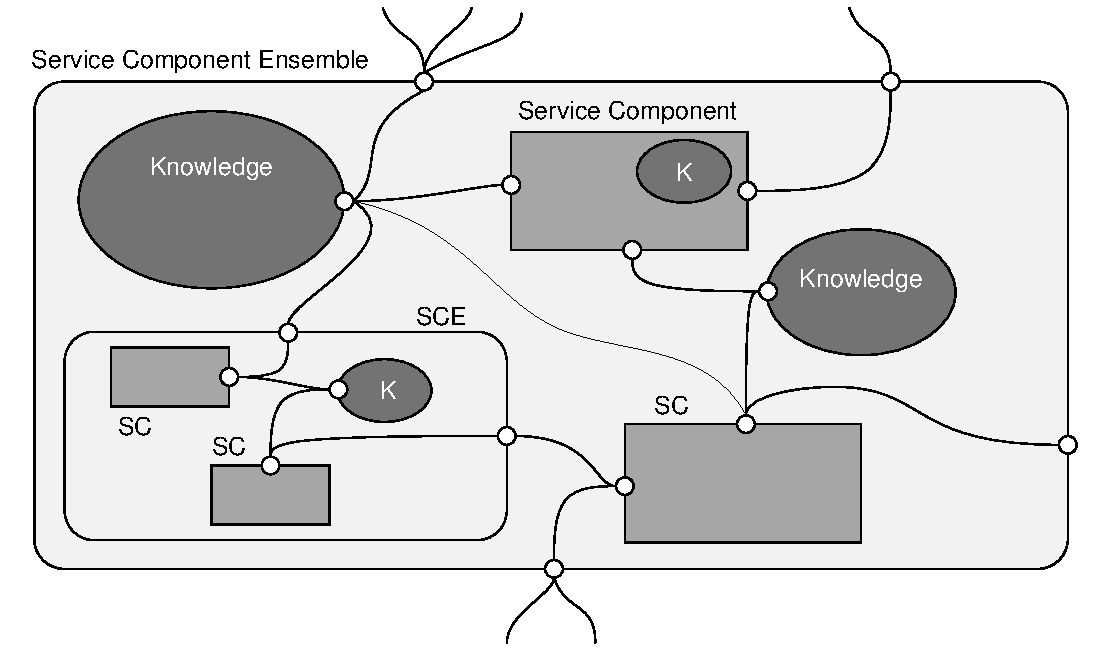
\includegraphics[width=8.2cm]{sce}
\vspace*{-.4cm}
\caption{A Service Component Ensemble}
\vspace*{-.3cm}
\label{ensemble}
\end{figure}

These notions of SCs and SCEs are the starting point of the EU project ASCENS~\cite{ascens,ASCENSatFMCO11} that aims at investigating different issues ranging from languages for modelling and programming SCEs to foundational models for adaptation, dynamic self-expression and reconfiguration, from formal methods for the design and verification of reliable SCEs to software infrastructures supporting deployment and execution of SCE-based applications. The aim is to develop formal tools and methodologies supporting the design of self-adaptive systems that can autonomously adapt to, also unexpected, changes in the operating environment, while keeping most of their complexity hidden from administrators and users.

In~\cite{SCEL} \SCEL{} (Service Component Ensemble Language), a new language designed for  autonomic computing has been presented. \SCEL\ brings together different programming abstractions that permit to directly represent \emph{knowledge}, \emph{behaviors} and \emph{aggregations} according to specific \emph{policies}. It also supports naturally programming self-awareness, context-awareness and adaptation. \SCEL's solid semantic grounds lay the basis for developing logics, tools and methodologies for formal reasoning about system behavior to establish qualitative and quantitative properties of both the individual components and the ensembles.

In this work we present \resp{} a Runtime Environment for \SCEL{} Programs that permits executing \SCEL{} programs. 
Our aim is to provide programmers with a framework that permits developing of autonomic and adaptive
systems according to the \SCEL{} paradigm. 

\section{\SCEL: design principles}
\label{sec:SCELtdesign}

\SCEL\ provides abstractions explicitly supporting autonomic computing systems in terms of \emph{Behaviors}, \emph{Knowledge} and \emph{Aggregations}, according to specific \emph{Policies}.

\emph{Behaviors} describe how computations progress. These abstractions are modelled as processes executing actions, in the style of standard process calculi. \emph{Interaction} comes in when components access data in the knowledge repositories of other components. \emph{Adaptation} emerges as the result of knowledge acquisition and manipulation.

\emph{Knowledge} provide the high level primitives to manage pieces of relevant information coming from different sources. Knowledge is represented through items stored in repositories. Knowledge items contain either \emph{application data} or \emph{awareness data}. The former are used for determining the progress of component computations, while the latter provide information about the environment in which the different components are running (e.g. monitored data from sensors) or about the actual status of an autonomic component (e.g. about its current position or the remaining battery's charge level). We assume that each knowledge repository's handling mechanism provides three abstract operations that can be used by autonomic components for \emph{adding} new knowledge to the repository, for \emph{retrieving} knowledge  from the repository and for \emph{withdrawing} knowledge from it.

\emph{Aggregations} describe how different entities are brought together to form \emph{components} and \emph{systems} and to offer the possibility to construct the \emph{software architecture} of autonomic systems. Composition of components and their interaction is implemented by exploiting the notion of \emph{interface} that can be queried to determine the attributes and the functionalities provided and/or required by components. \emph{Ensembles} are specific aggregations of components that represent \emph{social or technical networks} of autonomic components. The key point is that the formation rule is endogenous to components: components of an ensemble are connected by the interdependency relations established in their interfaces. Therefore, an ensemble is not a rigid fixed network but rather a dynamic graph-like structure where component linkages are dynamically established.

\emph{Policies} control and adapt the actions of the different components in order to guarantee the achievement of specific goals or the satisfaction of specific properties. Since few assumptions can be made about the operational environment, that is frequently open, highly dynamic and possibly hostile, the ability of programming and enforcing a finer control on behavior is essential to assure that e.g. valuable information is not lost. Policies are the mean to guarantee such control. Interaction policies and Service Level Agreement (SLA) policies provide two standard examples of policy abstractions. Other examples are security properties maintaining the right linkage between data values and their associated usage policies (data-leakage policies) or limiting the flow of sensitive information to untrusted sources (access control and reputation policies).

All these abstractions are aggregated by means of the notion of autonomic component. An \emph{autonomic component} $\loccomp{{\cal I}}{\knw,\pol,P}$ consists of:
\begin{enumerate}
\item an \emph{interface} \interf{I} publishing and making available structural and behavioral information about the component itself;
\item a \emph{knowledge manager} $\knw$, managing both application data and awareness data, together with the specific handling mechanism;
\item a set of \emph{policies} $\pol$ regulating the interaction between the different internal parts of the component and the interaction of the component with the others;
\item a \emph{process} $P$ together with a set of process definitions that can be dynamically activated. Some of the processes in $P$ perform local computation, while others may coordinate processes interaction with the knowledge repository and deal with the issues related to adaptation and reconfiguration.
\end{enumerate}

A component's interface can be inquired to extract information about the component, its status or its execution environment, as well as the services offered by the component. %The interface in fact provides an \emph{attribute} for each kind of information or provided service.
In fact, the interface provides a set of \emph{attributes} characterizing the component itself. Among these attributes, attribute $id$ is mandatory and is bound to the name of the component. Additional attributes might, e.g., indicate the battery's charge level and the component's GPS position. Suitable attributes are also used to indicate the provided services and their signature.
%\todo{Ros: should we give more details on how "provided services" are specified?\\}
Notably, the whole information provided by the component interface is stored in the local knowledge of the component and therefore can be dynamically manipulated by means of the operations provided by the knowledge repositories' handling mechanisms.

%\begin{remark}[Ensembles]
%Ensembles are sets of components characterized by means of suitable predicates over the attributes of components. Surprisingly (it might be), no specific syntactic category or operator for forming ensembles is provided by our language. Rather, to better capture their dynamicity, ensembles are `synthesized' dynamically by exploiting the values of the components attributes. This design choice guarantees high dynamicity and flexibility in forming, joining and leaving ensembles and does avoid resorting to structure ensembles through rigid syntactic constructs.
%\end{remark} 

\section{A runtime environment for \SCEL{} programs}
\label{sec:resp}

In this section we present \resp{}. This is a runtime environment that permits executing \SCEL{} programs. 
Our aim is to provide programmers with a framework that permits developing of autonomic and adaptive
systems according to the \SCEL{} paradigm. 

\paragraph{Design principles}

\SCEL{} aims at identifying linguistic constructs for uniformly modeling the control of computation, the interaction among possibly 
heterogeneous components, and the architecture of systems and ensembles.
%
A \SCEL{} \emph{program} consists of a set of components, each of which is equipped with its own knowledge repository, that
act and interact with each other. The number of components involved in the computation is not fixed but can change dynamically
during the computation. 
%
 \SCEL{} \emph{program} can be composed by a set of heterogeneous components that, relying on an highly dynamic communication
infrastructure,  concur  and cooperate to achieve a set of \emph{goals}.
%
That being on, a first principle that has driven the design and implementation of \resp{} has been to avoid \emph{centralised control}.
%
In particular, components can be able to interact with each other by simply relying on the available communication media.

In the definition of \SCEL{}, some categories, like \emph{knowledge} and \emph{policy}, are not fixed but these have to be fixed 
from time to time according to the specific application domain or to the taste of the language user. Other mechanisms, like for instance 
the underlying communication infrastructure, are not considered at all and \emph{abstracted} in the operational semantics. 
%
For this reasons, all the framework is parametric with respect to specific implementations of above mentioned features. Design patterns 
have been largely used in \resp{} to simplify development of specific implementations of knowledge, policies and underlying communication
infrastructure.

Finally, to simplify the integration with other tools/framework (like for instance Argos~\cite{??} and DEECo~\cite{??}), \resp{} relies on
 \emph{open technologies} like, for instance, \textsf{json}~\cite{JSON}. Such tools, providing mechanisms for data-interchange format,
simplify interactions between heterogeneous network components and provide the basis on which different runtime for 
 \SCEL{} programs can cooperate.
 
%\begin{enumerate}
%\item no centralized control
%\item heavy use of \emph{recurrent patterns} to simply 
%the development of specific
%\begin{itemize}
%\item policies
%\item knowledge
%\item \ldots
%\end{itemize} 
%\item use of \emph{open technologies} to support the integration with other tools/frameworks
%\begin{itemize}
%\item Argos
%\item DEECo
%\item \ldots
%\end{itemize}
%\end{enumerate}
%

\subsection{Components}
\label{sec:components}

The central element of \resp{} is the class \textsf{Node}. This class provides the implementation for a generic \SCEL{} component\footnote{From now on we will
use \emph{node} to refer to instances of class \textsf{Node}, while \emph{component} will indicate a \SCEL{} component.}.
%
The overall infrastructure of a generic node is reported in Figure~\ref{fig:respnode}. 

We assume that each node is executed over a virtual machine or a physical device that provides the access to: input and output devices
and network connections. 
%
Following the same structure considered in Section~\ref{sec:SCELtdesign}, each node contains:
\begin{itemize}
\item a \emph{knowledge}, described in Section~\ref{sec:knowledge};
\item a set of running processes/threads, described in Section~\ref{sec:agents};
\item a \emph{policy}, described in Section~\ref{sec:policies}.
\end{itemize}

Like for a \SCEL{} components, structural and behavioural information about a node 
can be collected into an \emph{interface}. This is rendered in \resp{} via a set of \emph{attribute collectors} (see
Section~\ref{sec:attributes}) that, reading values from the knowledge, publish and 
and make available attribute values in the interface.

Nodes interact with each other via \emph{ports} (Section~\ref{sec:ports}). These provide 
mechanism for supporting both \emph{one-to-one} and \emph{gruop} communications.  

%
%\SCEL{} aims at identifying linguistic constructs for uniformly modeling the control of computation, the interaction among possibly heterogeneous components, and the architecture of systems and ensembles. Therefore, we have left open some syntactic categories, namely
%%\textsc{Knowledge} (ranged over by $\knw$), \textsc{Policies} ($\pol$), \textsc{Templates} ($T$), and \textsc{Items} ($t$).
%\textsc{Knowledge}, \textsc{Policies}, \textsc{Templates} and \textsc{Items} (the last two ones determine the part of \textsc{Knowledge} to be added, retrieved or removed). These represent additional language features that need to be introduced, e.g. to represent and store knowledge of different forms (e.g. clauses, constraints, records, tuples) or to express a variety of policies (e.g. to regulate knowledge handling, resource usage, process execution, process interaction, actions priority, security, trust, reputation). We don't want to take a definite standing about these categories and prefer they be fixed from time to time according to the specific application domain or to the taste of the language user. In the rest of this section, we consider one by one the explicitly defined categories and describe them in detail.


\begin{figure}[tp]
	\begin{center}
	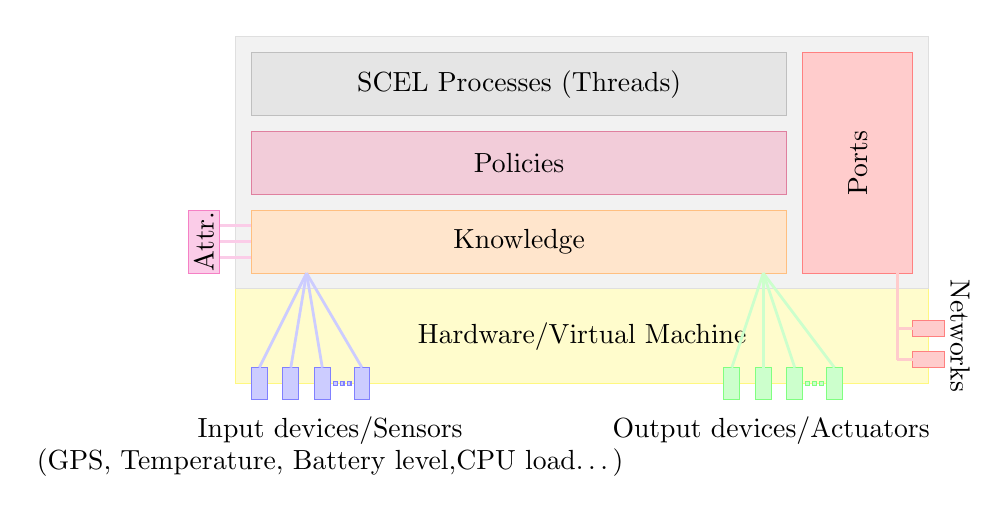
\begin{tikzpicture}[
         scale=.8%,font=\footnotesize,node distance=1cm and .1cm,
%      behavior/.style={rounded rectangle,thick,minimum size=.5cm,
%        draw=ASCENSBlue!65, solid,
%        top color=white, bottom color=ASCENSBlue!35,
%        text width=3cm,fill=white,text centered,drop shadow},
%      group/.style={fill=white,rotate=90,text width=6cm,text centered, draw,dashed,thick},
%      device/.style={rotate=90,text=black,minimum size=.5cm,
%        draw=ASCENSGrey1,very thick},    
%      external/.style={text=black,minimum size=.5cm, 
%        draw=ASCENSGrey1,very thick, left color=white,right color=rosso!40},
%      gui/.style={text=black,minimum size=.5cm, text width=3cm,text centered,
%        draw=ASCENSGrey1,very thick, left color=white,right color= dgreen!40},
%      sensor/.style={device,left color=white,right color=ASCENSGrey2},
%      actuator/.style={device,right color=white,left color=ASCENSGrey2},
%      tip/.style={->,very thick,draw=ASCENSGrey1}
      ]

	      \draw[draw=yellow!50,fill=yellow!20] (-5.5,0) rectangle (5.5,1.5);
	      \node[text centered] at (0,0.75) {Hardware/Virtual Machine};
	
	     \draw[draw=red!50,fill=red!20] (5.25,0.25) rectangle (5.75,.5);	
	     \draw[draw=red!50,fill=red!20] (5.25,0.75) rectangle (5.75,1.0);	
	     \node[text centered,rotate = -90] at (6.0,0.75) {Networks};

	     \draw[draw=blue!50,fill=blue!20] (-5.25,-.25) rectangle (-5.0,.25);	
	     \draw[draw=blue!50,fill=blue!20] (-4.75,-.25) rectangle (-4.5,.25);	
	     \draw[draw=blue!50,fill=blue!20] (-4.25,-.25) rectangle (-4.0,.25);	
	     \draw[draw=blue!50,fill=blue!20] (-3.95,-0.03) rectangle (-3.89,.03);	
	     \draw[draw=blue!50,fill=blue!20] (-3.84,-0.03) rectangle (-3.78,.03);	
	     \draw[draw=blue!50,fill=blue!20] (-3.73,-0.03) rectangle (-3.67,.03);	
	     \draw[draw=blue!50,fill=blue!20] (-3.62,-.25) rectangle (-3.37,.25);	
%	     \draw[draw=blue!50,fill=blue!20] (-4.25,-.25) rectangle (-4.0,.25);	
%	     \draw[draw=blue!50,fill=blue!20] (-4.25,-.25) rectangle (-4.0,.25);	
	      \node[text centered] at (-4,-0.75) {Input devices/Sensors};
	      \node[text centered] at (-4,-1.25) {(GPS, Temperature, Battery level,CPU load\ldots)};

	     \draw[draw=green!50,fill=green!20] (2.25,-.25) rectangle (2.5,.25);	
	     \draw[draw=green!50,fill=green!20] (2.75,-.25) rectangle (3.0,.25);	
	     \draw[draw=green!50,fill=green!20] (3.25,-.25) rectangle (3.5,.25);	
	     \draw[draw=green!50,fill=green!20] (3.55,-0.03) rectangle (3.61,.03);	
	     \draw[draw=green!50,fill=green!20] (3.66,-0.03) rectangle (3.72,.03);	
	     \draw[draw=green!50,fill=green!20] (3.77,-0.03) rectangle (3.83,.03);	
	     \draw[draw=green!50,fill=green!20] (3.88,-.25) rectangle (4.13,.25);	
%%	     \draw[draw=green!50,fill=green!20] (-4.25,-.25) rectangle (-4.0,.25);	
%%	     \draw[draw=green!50,fill=green!20] (-4.25,-.25) rectangle (-4.0,.25);	
	      \node[text centered] at (3,-0.75) {Output devices/Actuators};
%	      \node[text centered] at (-4,-1.25) {(GPS, Temperature, Battery level,CPU load\ldots)};


	      \draw[draw=lightgray!50,fill=lightgray!20] (-5.5,1.5) rectangle (5.5,5.5);

	      \draw[draw=gray!50,fill=gray!20] (-5.25,4.25) rectangle (3.25,5.25);
	      \node[text centered] at (-1,4.75) {SCEL Processes (Threads)};

	      \draw[draw=purple!50,fill=purple!20] (-5.25,3.0) rectangle (3.25,4.0);
	      \node[text centered] at (-1,3.5) {Policies};

	      \draw[draw=orange!50,fill=orange!20] (-5.25,1.75) rectangle (3.25,2.75);
	      \node[text centered] at (-1,2.25) {Knowledge};

	      \draw [draw=blue!20,line width=1pt] (-5.125,0.25) -- ( -4.375,1.75); 
	      \draw [draw=blue!20,line width=1pt] (-4.625,0.25) -- ( -4.375,1.75); 
	      \draw [draw=blue!20,line width=1pt] (-4.125,0.25) -- ( -4.375,1.75); 
	      \draw [draw=blue!20,line width=1pt] (-3.495,0.25) -- ( -4.375,1.75); 

	      \draw [draw=green!20,line width=1pt] (2.375,0.25) -- ( 2.875,1.75); 
	      \draw [draw=green!20,line width=1pt] (2.875,0.25) -- ( 2.875,1.75); 
	      \draw [draw=green!20,line width=1pt] (3.375,0.25) -- ( 2.875,1.75); 
	      \draw [draw=green!20,line width=1pt] (4.005,0.25) -- ( 2.875,1.75); 
	      
	      \draw[draw=magenta!50,fill=magenta!20] (-6.25,1.75) rectangle (-5.75,2.75);
	      \node[text centered,rotate=90] at (-6,2.25) {Attr.};
	      \draw [draw=magenta!20,line width=1pt] (-5.75,2.5) -- ( -5.25,2.5); 
	      \draw [draw=magenta!20,line width=1pt] (-5.75,2.25) -- ( -5.25,2.25); 
	      \draw [draw=magenta!20,line width=1pt] (-5.75,2) -- ( -5.25,2.); 

	      \draw[draw=red!50,fill=red!20] (3.5,1.75) rectangle (5.25,5.25);
	      \node[text centered,rotate=90] at (4.375,3.5) {Ports};
	
	      \draw [draw=red!20,line width=1pt] (5,1.75) -- ( 5,.375); 
	      \draw [draw=red!20,line width=1pt] ( 5,.375) -- ( 5.25,.375); 
	      \draw [draw=red!20,line width=1pt] ( 5,.875) -- ( 5.25,.875); 
	      
	      \node at (5.5,5.5) {$\ $};
	    
	
	\end{tikzpicture}
    	\end{center}
	\caption{Node architecture}
	\label{fig:respnode}
\end{figure}

\subsection{Knowledge}
\label{sec:knowledge}

The interface \textsf{Knowledge}\footnote{All the classes considered in this section are part of package \resppackage{knowledge}.},
identifies a generic \emph{knowledge repository} and provides the high level primitives to 
manage pieces of relevant information coming from different sources. 
%
This interface is contains the following methods:
\begin{itemize}
\item \textsf{put( Tuple t ): boolean}
\item \textsf{get( Template t ): Tuple}
\item \textsf{getp( Template t ): Tuple}
\item \textsf{query( Template t ): Tuple}
\item \textsf{queryp( Template t ): Tuple}
\end{itemize}

Method \textsf{put} adds a tuple to the knowledge and returns a boolean value
indicating if the operations has been successfully executed or not. 
%
Class \textsf{Tuple}, defined in the same package of \textsf{Knowledge}, identifies the basic information item. It consists
of a sequence of values, i.e. \textsf{Objects}, that can be collected into a knowledge repository.

The other methods, that can be used to retrieve knowledge items from a knowledge repository, 
take as parameter an instance of \textsf{Template}. This is used to select elements in a knowledge repository
and consists of is a sequence of \textsf{TemplateField}. 
%
A \textsf{TemplateField} is an interface containing 
the following single method:
\begin{itemize}
\item \textsf{match( Object o ): boolean}
\end{itemize}
%
Class \textsf{Template} relies on this method to verify if a \textsf{Tuple} can be selected or not. Indeed, a tuple
matches a template if both the object have the same length and the corresponding element 
matches.

Let \textsf{k} be a \textsf{Knowledge}. Method \textsf{k.get( t )} is used to remove a tuple matching template \textsf{t} 
from the knowledge \textsf{k}. This is a blocking operation. Indeed, the thread invoking the method is blocked
until a tuple matching \textsf{t} is not found. Method \textsf{k.query(t)} is similar. However, while with \textsf{get}
the matching tuple is physically removed from the knowledge, with \textsf{query} this is only read. Moreover,
implementation of interface \textsf{Knowledge} can provide mechanisms to \emph{infer} tuples according to
the actual value in knowledge. 

Finally, methods \textsf{getp} and \textsf{queryp} are the predicative variants of \textsf{get} and \textsf{query}.
Namely, \textsf{getp} and \textsf{queryp} are not blocking operations: if a \textsf{k.getp( t )} (respectively \textsf{k.queryp( t )}) is 
executed when a tuple matching \textsf{t} is not in the knowledge, value \textsf{null} is returned.  

Currently, a single implementation of interface \textsf{Knowledge} is available in \resp{}. Class
\textsf{TupleSpace} in package \resppackage{knowledge.ts} provides an implementation
for a Linda~\cite{Gel85} tuple space. 

\subsection{Sensors} 
\label{sec:sensors}

To retrieve data from external input devices, nodes can be equipped with \emph{sensors}. These
are instances of class \textsf{Sensor} that can be used to identify a generic source of information.
%
Each sensor can be associated to a logical or physical device providing data that
can be used by processes and that can be the subject of adaptation.

Each sensor exports data as a \emph{tuple}. We will see below that the same actions used 
to retrieve values from knowledge, namely \textsf{query}, can be used to obtain data from a 
sensor. In fact, each node \emph{hides} the real source of information to processes.

%\begin{itemize}
%\item it can be associated to a logical/physical sensor
%\item values are exported as a \emph{tuple}, each implementation has to define the structure of the tuple containing
%\begin{itemize}
%\item \textsf{(``GPS", 45.8 , 37.2)}
%\item \textsf{(``BATTERY" , \%87)}
%\end{itemize}
%\item \textsf{query} actions are used to \emph{retrieve} data from sensor
%\end{itemize}

\subsection{Actuators} 
\label{sec:actuators}

Instances of class \textsf{Actuator} can be used to send data to external components or devices.
Similarly to \textsf{Sensor}, an instance of class \textsf{Actuator} can be used to \emph{control}
an \emph{external} component  that identify a logical/physical actuator. 
%
Processes can pass values to actuators by relying on standard \SCEL{} operations.
%
%Abstract class \textsf{Actuator} is used to identify an external device that can be controlled
%by SCEL processes:
%\begin{itemize}
%\item it can be associated to a logical/physical actuator
%\item values are passed as a \emph{tuple}, each implementation has to define the structure of the tuple containing
%\begin{itemize}
%\item \textsf{(``DIRECTION", $\pi/3$)}
%%\item \textsf{(``BATTERY" , \%87)}
%\end{itemize}
%\item values are passed to a actuator via \textsf{put} actions
%\end{itemize}

\subsection{Attributes and Atribute collectors} 
\label{sec:attributes}

An attribute is defined as a pair \emph{(name,value)}. Attributes can be published in a node
interface via \emph{attribute collectors}. 
%
Attribute collectors can be implemented by extending abstract class \textsf{AttributeCollector}.
%
This class has \textsf{protected} fields:
\begin{itemize}
\item \textsf{name: String}, containing the name associated to the published attribute;
\item \textsf{template: Template}, identifying the template used to retrieve the knowledge element
that will be used to compute actual attribute value.
\end{itemize}

When a node receives a request for an attribute \emph{a}, a collector with the same name is
selected. Hence, a tuple matching the template associated to the collector is retrieved from 
the knowledge. If an attribute with name \emph{a} does not exists, or a tuple matching the
collector template is not available in the knowledge, an attribute with value \textsf{null} is returned.
Otherwise, the (abstract) method \textsf{doEval} is used to compute the actual 
attribute value (subclasses of \textsf{AttributeCollector} has to provide an implementation for this method).

\subsection{Ports and network infrastructure}
\label{sec:ports}

Each node is equipped with a set of \emph{ports} that are 
able to handle both  \emph{point-to-point} interactions and \emph{group} interactions (\emph{ensemble} oriented).
%
Indeed, a port provides a generic communication channel that follow a specific communication protocol. 

Currently the following ports have been developed:
\begin{itemize}
\item \textsf{InetPort}, this kind of ports uses TCP to \emph{point-to-point} interactions and UDP for the \emph{group} ones;
\item \textsf{ServerPort}, in this case a centralized server is used to collect and dispatch nodes' actions;
\item \textsf{VirtualPort}, this is used to \emph{simulate} nodes running on \emph{virutal} devices.
\end{itemize} 

To simplify interactions with other framework/tools, even developed in languages that are different from
\java{}, messages are sent using a \textsf{json} format.

Each port is identified by a physical address. For instance, in the case of \textsf{InetPort} this is the 
\emph{inet-address} associated to the socket where a thread is waiting for incoming connections.

%
%\paragraph{Esempio:} $\acgetp T \enspred{P}$ 
%\begin{enumerate}
%\item A request message containing template $T$ and attribute names occurring in $\enspred{P}$ is sent
%via a \emph{multicast} channel
%\item All the components that receives the message reply with:
%\begin{itemize}
%\item a tuple $t$ matching template $T$
%\item a list of requested attributes 
%\end{itemize}
%\item If the node originating the requests receives attributes that \emph{satisfies} predicate $\enspred{P}$, action is executed. Otherwise,
%the request is sent again. 
%\end{enumerate}


\subsection{Agents}
\label{sec:agents}

Agents are the \resp{} active computational units and are threads used to program the behaviour of 
\SCEL\  processes. Class \textsf{Agent} is an abstract class providing the following methods:
\begin{itemize}
\item \textsf{abstract doRun(): void}
\item \textsf{put(Tuple, Target): boolean}
\item \textsf{get(Template, Target): Tuple}
\item \textsf{getp(Template, Target): Tuple}
\item \textsf{query(Template, Target): Tuple}
\item \textsf{queryp(Template, Target): Tuple}
\item \textsf{exec( Agent a ): boolean}
\end{itemize}

%Each process is built up from the \emph{inert} process $\procnil$ via \emph{action prefixing} ($a.P$), 
%\emph{nondeterministic choice} ($P_1 \choice P_2$), \emph{controlled composition} ($\auth {P_1} {P_2}$), 
%\emph{process variable} ($X$), \emph{parameterised process invocation} ($A(\bar{p})$), and 
%\emph{parameterised process definition} ($A(\bar{f}) \define P$). The construct $\auth {P_1} {P_2}$ abstracts the 
%various forms of parallel composition commonly used in process calculi. Process variables are used to support 
%higher-order communication, namely the capability to exchange (the code of) a process by first adding an item 
%containing the process to a knowledge repository and then retrieving/withdrawing this item while binding the process to a process variable.

The first method is the one subclasses has to implement in order to define agent behaviour. This method is invoked
when the agent starts is computation. 
%
Methods \textsf{put}, \textsf{get}, \textsf{getp}, \textsf{query} and \textsf{query} are used to manage shared knowledge 
repositories by withdrawing/retrieving/adding information items from/to a knowledge repository.
These methods extend the one considered in Section~\ref{sec:knowledge} by with another parameter
identifying the, possibly remote, node where the target knowledge repository is located.

A target can be either a \emph{point-to-point} address, a \emph{group} or \emph{self}. 
%
A point-to-point address univocally identify the target of the considered action.  A \emph{group} 
identifies all the nodes that satisfy a given predicate on nodes attributes. Special target \textsf{Self} 
is used to refer to the node where an agent is running.
%
The classes implementing the possible target, in conned in package \resppackage{topology}, are \textsf{PointToPoint}, \textsf{Group} and 
\textsf{Self}, respectively.

%%. These operations exploit templates $T$ as patterns to select knowledge items $t$ in the repositories. They rely heavily on the used 
%%knowledge repository and are implemented by invoking the handling operations it provides. Action $\acexecp P$ triggers a controlled (parallel) 
%%execution of process $P$. Action $\acnewp {\interf{I},\knw,\pol,P}$ creates a new component $\loccomp{{\cal I}}{\knw,\pol,P}$.
%
%Action $\acget$ is a \emph{blocking} action, in the sense that the process executing it has to wait for the wanted element if it is not (yet) available in the knowledge repository. Action $\acread$, exactly like $\acget$, suspends the process executing it if the knowledge repository does not (yet) contain or cannot `produce' the wanted element. The two blocking actions differ also for the fact that $\acget$ removes the found item from the knowledge repository while $\acread$ leaves the target repository unchanged. Actions $\acput$, $\acexec$ and $\acnew$ are instead non-blocking and are immediately executed (provided that their execution is allowed by the policies in force).
%
%Component names are denoted by $\naddr$, $\naddr'$, \ldots, variables for names are denoted by $\vaddr$, $\vaddr'$, \ldots, while $\nvaddr$ stands for a name or a variable. The distinguished variable $\self$ can be used by processes to refer to the name of their hosting component. $\enspred{P}$ can be either a predicate over attributes or the name of a predicate; in the latter case, the association between the name and the predicate is stored as an attribute (defined in the interface) of the component.
%%\todo{Is it useful having predicates with more than one argument as e.g. $\enspred{P}(I,J,...)$? If yes, it is reasonable to have arguments different from interfaces?\\}
%
%In actions of the form $\acputp t {\enspred{P}}$, predicate $\enspred{P}$ acts as a `guard' specifying \emph{all} the components that may be affected by the execution of the action, i.e. the target must satisfy the guard in order for the action to take place. Thus, actions $\acputp t n$ and $\acputp t {\enspred{P}}$ give rise to two different primitive communication forms: the former is a point-to-point communication, while the latter is a sort of group-oriented communication. The set of components satisfying $\enspred{P}$ can be considered as the \emph{ensemble} which the process performing the action is willing to interact with.
%%
%For example, the names of the components that can be members of an ensemble can be fixed via the predicate
%\[
%\enspred{P}(\interf{I})\defi\interf{I}.id \in \set{n,m,p}
%\]
%If the predicate above is used as the target of a communication action, then that action will act on those components whose name is $n$, $m$ or $p$, if any.
%%
%As another example, to dynamically characterize the members of an ensemble that are active and have a battery charge level greater than 30\%, the predicate
%\[
%\enspred{P}(\interf{I})\defi\interf{I}.active = yes \wedge {\cal I}.battery\_level > 30\%
%\]
%could be used. Here, we are assuming that the interface of each component willing to be part of the ensemble contains the attributes $active$ and $battery\_level$.

\subsection{Policies}
\label{sec:policies}

\emph{Policies} are attached to a node in order to control and adapt the performed actions to guarantee the achievement of specific 
goals or the satisfaction of specific properties. In particular, when an agent invokes a method, this is first delegated to the policy 
associated to the associated policy. This guarantee that \SCEL{} action execution is appropriately regulated.

The interface \textsf{Policy} provides methods of the form:
\begin{itemize}
\item \textsf{put(Agent a, Tuple t , Target l)}
\item \textsf{acceptGet( Locality l , Template t )}
\end{itemize}

The first one is used when agent \textsf{a} executes an action (in this case a \textsf{put}). While the second one is
used  to control the actions executed by remote components (in this case a \textsf{get}).

Policies are organized in a \emph{stack}. The policy at one level relies on the one at the level below to
actually execute \SCEL{} actions. The policy at the lower level is the one that allows any operation.


\section{\resp{} at work}
\label{sec:atwork}


We now use \SCELTS{} to model a swarm robotic scenario where the robots in the swarm have to reach 
a \emph{safe area}. Not all the robots have to reach the same goal. Indeed, 
each robot is identified by a colour that can be either \emph{red} or \emph{green}. Red robots have to
reach the read area, while green robots have to reach the green one. 

Robots are distributed over a physical area and are not informed about the position of the two target zones. For
this reason, to discover the location of target, each robot follows a \emph{random walk}. As soon as a robot reaches the area, it publishes 
its location in the local knowledge repository. In this way, robots with the same colour can get informed 
about the location of the corresponding target. Notice that, by relying on \emph{group} queries, the identity of the 
robot publishing the target location can be ignored. Informed robots can then
move directly towards the target.

We model each robot as a \SCELTS{} component\footnote{In the rest of this section we will use the terms robot, component or node to identify the \SCEL{} 
components associated to each robot in the scenario.}. To identify the two kind of robots, we use attribute \textsf{colour}. Hence,
let $\interf{I}$ be the robot interface, we have that $\interf{I}.\textsf{colour}=col$ if and only if 
a tuple of the form:
%
\[
\tuple{ attribute , ``\mathsf{colour}", col }
\]
%
is part of the local knowledge repository.

We also assume that robots are equipped with a GPS sensor and with 
a sensor that permits verifying if the target area has been reached or not. These sensors publish 
their value directly on the knowledge repository. Namely, a tuple of the form $\tuple{ ``\textsf{GPS}" , x , y }$ is
in the local tuple-space if the robot is located at $(x,y)$. Similarly, a tuple $\tuple{ ``\textsf{TARGET}" , \textsf{true} }$ 
is in the robot tuple-space if and only if the goal area has been reached. Conversely, a tuple
$\tuple{ ``\textsf{TARGET}" , \textsf{false} }$ indicates that the robot has to yet reached the goal area.
%
The above mentioned tuples are generated by the physical components that are able to read the GPS values
and to verify the \emph{colour} of the floor under the robot. 

Three processes run at each robot:
\begin{itemize}
\item \textsf{randomWalk}, that controls robot movements while it is discovering the goal area;
\item \textsf{targetSeeker}, that verifies if the target area has been reached;
\item \textsf{dataSeeker}, that tries to retrieve data from other robots with the same colour in order to
obtain the actual position of the target goal area.
\end{itemize}

The code of \textsf{randonWalk} process is the following\footnote{In the code we use high level programming constructs,
like \textsf{if}-\textsf{then}-\textsf{else} or \textsf{while}, that can be easily implemented
as macro in the \SCELTS{}}:

\begin{center}
\begin{tabular}{l}
\textsf{while} ($\neg found\wedge\neg informed$) \{ \\
\quad \color{gray}{\% sends value to an actuator to indicate the direction}\\
\quad $\acputp{ \mbox{ ``\textsf{DIRECTION}'' } , random()\cdot 2\pi }{\self}.$ \\
\quad \color{gray}{\% reads from the \emph{target} sensor if the safe-area has been reached }\\
\quad $\acreadp{ \mbox{``TARGET''} , ?found }{\self}.$\\
\quad \color{gray}{\% checks if the robot is informed about the safe-area location}\\
\quad $\acreadp{ \mbox{``INFORMED''} , ?informed}{\self}.$\\  
\}
\end{tabular}
\end{center}

This process randomly selects a  direction where the robot moves to search the target area.
This operation is performed by adding tuple 
%
\[
\tuple{ \mbox{ ``\textsf{DIRECTION}'' } , random()\cdot 2\pi }
\]
%
in the local tuple-space. We assume that this tuple will be retrieved by a physical component governing
the robot wheels. 
%
Process \textsf{randonWalk} is executed until the robot falls into the goal area or the robot is informed (i.e. the actual
position of the target area has been obtained from another robot). These conditions are verified
by retrieving tuples $\tuple{ \mbox{``TARGET''} , ?found }$ and tuple $\tuple{ \mbox{``INFORMED''} , ?informed }$.
%
These tuples are always available and controlled by the \emph{target sensor} outlined above
and by process \textsf{dataSeeker} that will be described in few paragraphs. 

Process \textsf{targetSeeker} checks if the target area has been reached and, in the case, publishes actual
robot position and stops robot movement. The code of process \textsf{targetSeeker} is the:

\begin{center}
\begin{tabular}{l}
\textsf{while} ($\neg found$) \{ \\
\quad \color{gray}{\% reads from the \emph{target} sensor if the safe-area has been reached }\\
\quad $\acreadp{ \mbox{``TARGET''} , ?found }{\self}.$\\
\quad \textsf{if} ($found$) \{\\
\quad\quad \color{gray}{\% sends value to an actuator to stop the robot}\\
\quad\quad $\acputp{ \mbox{ ``STOP''} }{\self}.$\\
\quad\quad \color{gray}{\% retrieves current position from GPS}\\
\quad\quad $\acreadp{ \mbox{``GPS''} , ?x , ?y }{\self}.$\\
\quad\quad \color{gray}{\% publishes the location in the local knowledge}\\
\quad\quad $\acputp{ \mbox{ ``TARGET\_LOCATION''} , x , y }{\self}.$\\
\quad\}\\
\}
\end{tabular}
\end{center}

The process above guarantees that when the robot reaches the target, tuple 
$\tuple{\mbox{ ``TARGET\_LOCATION''} , x , y}$ is added to the local knowledge repository ($x$
and $y$ identifies the robot position). This tuple can be retrieved by other robots of the same
colour. These will not follow anymore a random walk but will move directly towards the 
target area. 
%
This task is performed by process \textsf{dataSeeker}, defined below, by relying on 
\emph{group communication} (below, variable $col$ identifies robot colour):

\begin{center}
\begin{tabular}{l}
 \color{gray}{\% retrieves target location from any robot! }\\
 $\acreadp{ \mbox{``TARGET\_LOCATION''} , ?x , ?y}{\{\mathsf{\interf{I}.\textsf{color}=col}\}}.$\\
 \color{gray}{\% publishes the location in the local knowledge}\\
 $\acputp{ \mbox{ ``TARGET\_LOCATION''} , x , y }{\self}.$\\
 \color{gray}{\% updates the local information (the robot is now \emph{informed}) }\\
 $\acreadp{ \mbox{``INFORMED''} , \mathsf{false} }{\self}.$\\  
 $\acreadp{ \mbox{``INFORMED''} , \mathsf{true} }{\self}.$\\  
 \color{gray}{\% sets the right directin towards the safe-area }\\
 \textsf{while} ($\neg found$) \{ \\
 \quad $\acputp{ \mbox{ ``DIRECTION'' } , towards(x,y) }{\self}.$ \\
 \quad $\acreadp{ \mbox{``TARGET''} , ?found }{\self}.$\\
 \}
\end{tabular}
\end{center}

%%%%%
In this section we present a simple example that shows how \resp{} can be used to
support development and execution of \SCEL{} systems.
%
We consider a set of robots have to reach a safe-area.  To discover the location of safe-area, 
each robot follows a \emph{random walk}. As soon as a robot reach the area, it publishes locally its location 
in the local knowledge repository. Thanks to By relying on \emph{group} queries, other robots can get informed 
about the location of the safe-area and then can move directly to the target.

We assume that each robot is equipped with  a GPS sensor, 
a sensor to verify if the target are has been reached or not. Moreover, to control
 movement, we assume that each robot is equipped with an actuator to change direction
 and with an actuator to stop movement.
 
 To implement this scenario we let each robot be implemented as a SCEL component. To
 permits simulating the scenario we a virtual port to handle robot communication and
 an ad-hoc data structure to take care of robot position and movement.
 
\begin{center}
%\begin{center}
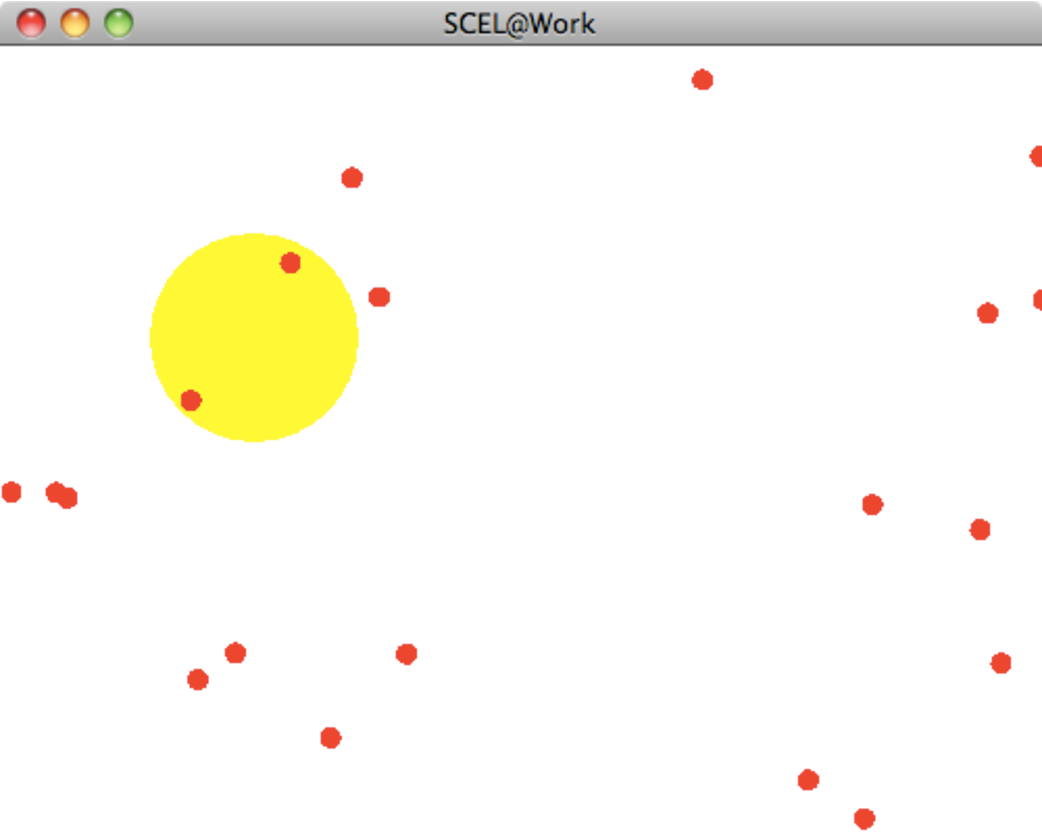
\includegraphics[scale=0.25]{img/scenariosimple}
%\end{center}
%\end{tabular}
\end{center}

\begin{center}
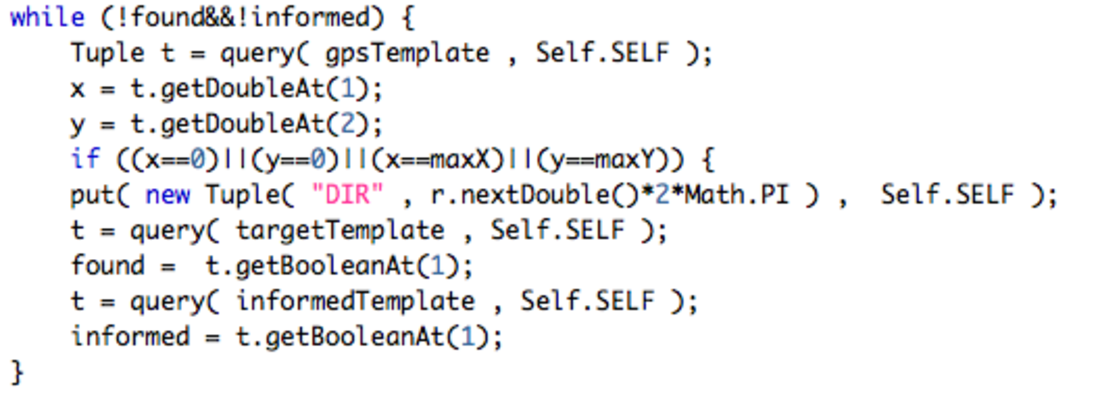
\includegraphics[scale=0.5]{img/pieceofcode}
\end{center}

\begin{center}
%\begin{center}
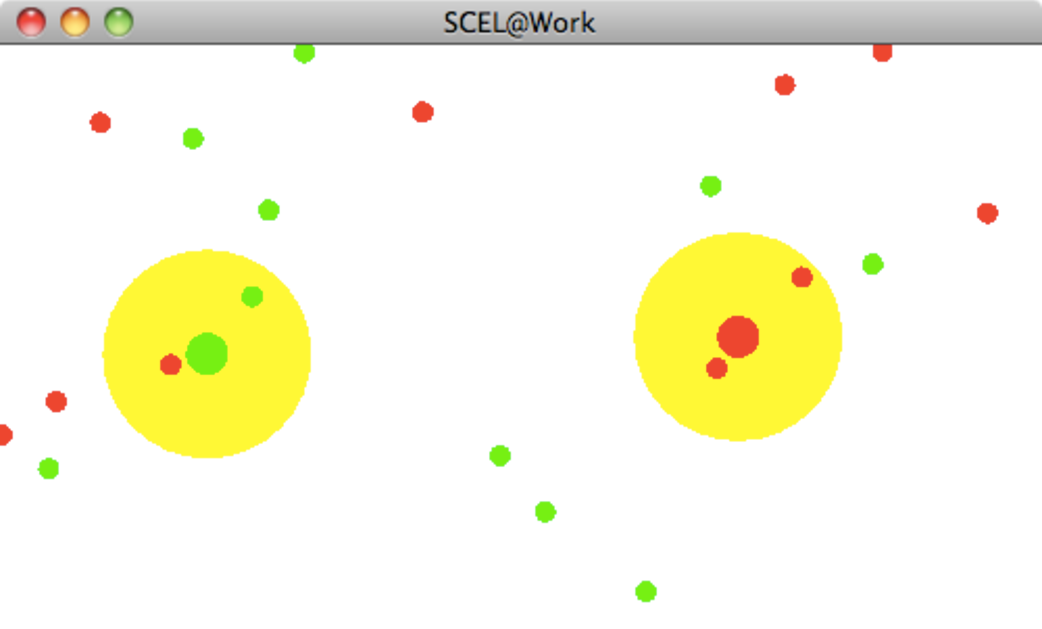
\includegraphics[scale=0.45]{img/doublemobility}
%\end{center}
%\end{tabular}
\end{center}

\begin{center}
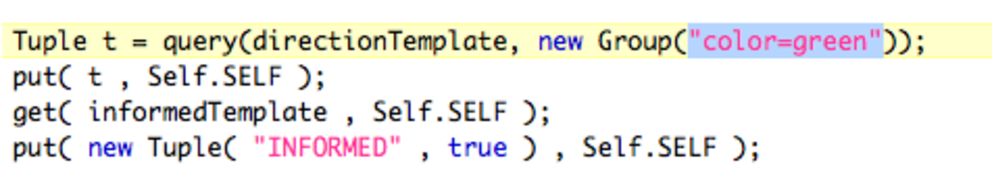
\includegraphics[scale=0.45]{img/groupcode}
\end{center}


\section{Conclusions} 

We have presented (first version of) a framework that permits developing and
executing \SCEL{} oriented applications in \java{}.

Considered framework should be now \emph{populated} with
specific implementations for \emph{policies}, \emph{knowledge}. 

Moreover, we plan to develop examples that, starting from Ascens case studies, can be used to \emph{validate}
the proposed solutions.

We are now working on a \emph{top-level} programming language that, enriching SCEL
with standard programming primitives, permits simplifying development of SCEL programs.

\bibliographystyle{splncs}
\bibliography{biblio}

\end{document}
